	\chapter{}
\label{lecture2}

\noindent На прошлой лекции мы установили, что минимайзер в задаче на $\min\limits_{y\in\K}\,\J[y]$, где  $\J[y]=\int\limits_a^b F(x,y,y')\,dx$ $\K=\left\{y(x)|y\in\Cfn[{[a,b]}]{1}, y(a)=y_0, y(b)=y_1, |y|<M\right\}$ удовлетворяет уравнению Эйлера--Лагранжа:
\begin{equation}
	\label{l2:eq:1}
	\hfill F_y-\der{}{x}F_{y'}=0,\hfill
\end{equation} 
которое надо решать при условиях 
\begin{equation}
	\label{l2:eq:2}
	\hfill y(a)=y_0,\ y(b)=y_1\hfill
\end{equation}

\section{Примеры решения уравнения Эйлера--Лагранжа.}
\label{lecture2section1}
Рассмотрим следующие частные случаи.
\begin{enumerate1}
	\item \label{l2:1:enum1} $F=F(x,y)$ --- нет зависимости от $y'$. Уравнение \eqref{l2:eq:1} принимает вид $F_y=0$, откуда при $F_{yy}\neq0$ можно по теореме о неявной функции найти $y=y(x)$. Так как функция $y(x)$ не содержит свободных констант, то в общем случае\footnote[1]{Здесь важно, что именно в \emph{общем случае}. Поскольку задача могла быть придумана хитрыми составителями задачников таким образом, чтобы решение удовлетворяло условиям $y(a)=y_0,\  y(b)=y_1$.} $y(a)\neq y_0$, $y(b)\neq y_1$, то есть решения нет. 
	
	\item  $F=\alpha(x,y)\cdot y'+\beta(x,y)$ --- функция линейна по $y'$. Уравнение Эйлера в этом случае
	\begin{equation}
		\label{l2:eq:3}
		\alpha_y\cdot y'+\beta_y-\der{}{x}\alpha(x,y)=\underline{\alpha_y\cdot y'}+\beta_y-\alpha_x-\underline{\alpha_y\cdot y'}=\beta_y-\alpha_x=0
	\end{equation}
	Далее возможны два варианта. Первый $\beta_y-\alpha_x=0$ не тождественно, то есть \eqref{l2:eq:3} можно рассматривать как уравнение относительно $y$ и мы приходим к \ref{l2:1:enum1}: в общем случае решения нет. 
	\noindent Второй вариант: $\beta_y-\alpha_x\equiv0$, то есть уравнения нет и, значит, любая кривая из \K --- экстремаль. Но при $\beta_y=\alpha_x$ можно указать такую функцию $\widetilde{\phi}(x,y)$ так, что $\alpha(x,y)=\widetilde{\phi}_y$, $\beta(x,y)=\widetilde{\phi}_x$ и интегрант $\alpha(x,y)\cdot y'+\beta(x,y)=\displaystyle\der{\widetilde{\phi}}{x}$. Поэтому 
	\begin{equation*}
		\int\limits_a^b(\alpha\cdot y'+\beta)\,dx=\int\limits_a^b\der{\widetilde{\phi}}{x}(x,y)\,dx=\widetilde{\phi}(b,y(b))-\widetilde{\phi}(a,y(a))=\widetilde{\phi}(b,y_1)-\widetilde{\phi}(a,y_0).
	\end{equation*}
	Таким образом значение интеграла не зависит от функций $y(x)\in\K$ и задача на $\min\limits_{y\in\K}\,\J[y]$ и $\max\limits_{y\in\K}\,\J[y]$ не имеет смысла.
	
	\item $F=F(y')$. Уравнение $\der{}{x}F_{y'}=0\rightarrow F_{y'}=const$ и при $F_{y'y'}\neq0$ мы получаем, что $y(x)=c_1\cdot x+c_2$, где константы $c_1$ и $c_2$ находятся из граничных условий.
	
	\item $F=F(y,y')$ --- нет явной зависимости от аргумента $x$, зависимость только через $y(x)$, $y'(x)$. Это наиболее часто встречающийся частный случай. Покажем, что в этом случае уравнение Эйлера имеет первый интеграл
	\begin{equation}
		\label{l2:eq:4}
		\hfill F-y'\cdot F_{y'}=const.\hfill
	\end{equation}
	То есть убедимся, что на любом решении $y=y(x)$ уравнения \eqref{l2:eq:1} выполняется \eqref{l2:eq:4}. Проверим \eqref{l2:eq:4}, подставив туда произвольную функцию $y(x)$, удовлетворяющую \eqref{l2:eq:1}, и взяв полную производную по $x$ от левой части \eqref{l2:eq:4}. Получим
	\begin{equation*}
		F_y\cdot y'+\underline{F_{y'}\cdot y''}-\underline{y''\cdot F_{y'}}-y'\cdot\der{}{x}F_{y'}=y'\underbrace{\left(F_y-\der{}{x}F_{y'}\right)}_{\text{левая часть \eqref{l2:eq:1}}}\equiv0. 
	\end{equation*} 
	Значит левая часть \eqref{l2:eq:4} --- действительно константа при $y$ из \eqref{l2:eq:1}.
	\vspace{0.2cm}
	
	\noindent\textbf{Задание. }Пусть \eqref{l2:eq:4} выполняется. Могут ли у уравнения \eqref{l2:eq:4} быть решения, не удовлетворяющие \eqref{l2:eq:1}?  
\end{enumerate1}

\section[Задачи для функционалов, зависящих от вектор-функций.]{Вариационные задачи для функционалов, зависящих от {\itshape n} функций одной переменной.}
\label{lecture2section2}
%\makeatletter
%\renewcommand{\@oddhead}{\hfill\thepage}
%\makeatother
Сейчас мы будем рассматривать функционалы вида 
\begin{equation*}
	\hfill\J[y_1,\ldots,y_n]=\int\limits_a^b F(x,y_1,\ldots,y_n,y'_1,\ldots,y'_n)\,dx\hfill
\end{equation*}

Приведём пример задачи, в которой возникает необходимость найти минимум функционала подобного рода. Пусть $A(a_0,b_0,c_0)$ и $B(a_1,b_1,c_1)$ --- произвольные точки и в точке $A$ помещён источник света.

\tikzset{every picture/.style={line width=0.75pt}} %set default line width to 0.75pt        

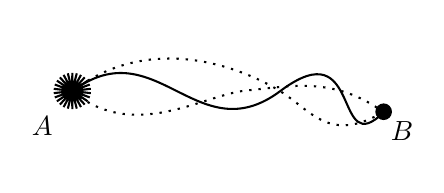
\begin{tikzpicture}[x=0.75pt,y=0.75pt,yscale=-1,xscale=1]
	%uncomment if require: \path (0,80); %set diagram left start at 0, and has height of 80
	
	%Shape: Star [id:dp7216217040010413] 
	\draw  [color={rgb, 255:red, 0; green, 0; blue, 0 }  ,draw opacity=1 ][fill={rgb, 255:red, 208; green, 2; blue, 27 }  ,fill opacity=1 ] (50,18) -- (50.03,26.5) -- (52.15,18.25) -- (50.09,26.52) -- (54.18,19) -- (50.15,26.54) -- (55.97,20.2) -- (50.19,26.58) -- (57.41,21.78) -- (50.23,26.63) -- (58.42,23.65) -- (50.25,26.69) -- (58.93,25.7) -- (50.26,26.75) -- (58.93,27.8) -- (50.25,26.81) -- (58.42,29.85) -- (50.23,26.87) -- (57.41,31.72) -- (50.19,26.92) -- (55.97,33.3) -- (50.15,26.96) -- (54.18,34.5) -- (50.09,26.98) -- (52.15,35.25) -- (50.03,27) -- (50,35.5) -- (49.97,27) -- (47.85,35.25) -- (49.91,26.98) -- (45.82,34.5) -- (49.85,26.96) -- (44.03,33.3) -- (49.81,26.92) -- (42.59,31.72) -- (49.77,26.87) -- (41.58,29.85) -- (49.75,26.81) -- (41.07,27.8) -- (49.74,26.75) -- (41.07,25.7) -- (49.75,26.69) -- (41.58,23.65) -- (49.77,26.63) -- (42.59,21.78) -- (49.81,26.58) -- (44.03,20.2) -- (49.85,26.54) -- (45.82,19) -- (49.91,26.52) -- (47.85,18.25) -- (49.97,26.5) -- cycle ;
	%Curve Lines [id:da67657481940421] 
	\draw  [dash pattern={on 0.84pt off 2.51pt}]  (50,26.75) .. controls (90,-3.25) and (135,17.5) .. (150,26.75) .. controls (165,36) and (174,52.5) .. (200,36.75) ;
	%Shape: Circle [id:dp7965230360360749] 
	\draw  [fill={rgb, 255:red, 0; green, 0; blue, 0 }  ,fill opacity=1 ] (196.5,36.75) .. controls (196.5,34.82) and (198.07,33.25) .. (200,33.25) .. controls (201.93,33.25) and (203.5,34.82) .. (203.5,36.75) .. controls (203.5,38.68) and (201.93,40.25) .. (200,40.25) .. controls (198.07,40.25) and (196.5,38.68) .. (196.5,36.75) -- cycle ;
	%Curve Lines [id:da7368235583824736] 
	\draw    (50.26,26.75) .. controls (90.26,-3.25) and (110.26,56.75) .. (150.26,26.75) .. controls (190.26,-3.25) and (175.26,61.75) .. (200.26,36.75) ;
	%Curve Lines [id:da9133689246774286] 
	\draw  [dash pattern={on 0.84pt off 2.51pt}]  (50.03,27) .. controls (80,51.5) and (113,28.5) .. (134,26.5) .. controls (155,24.5) and (176,19.5) .. (200.03,37) ;
	
	% Text Node
	\draw (29,37.4) node [anchor=north west][inner sep=0.75pt]    {$A$};
	% Text Node
	\draw (202,40.15) node [anchor=north west][inner sep=0.75pt]    {$B$};
	
	
\end{tikzpicture}

\noindent Надо определить траекторию луча от $A$ к $B$. Согласно принципу Ферма, свет распространяется по кривой, по которой время его прохождения от $A$ к $B$ меньше (или равно) времени распространения по близким кривым. Пусть $\Gamma=\{x(s),y(s),z(s)\}$ --- произвольная кривая, соединяющая точки $A$~(при $s=s_0$) и $B$ (при $s=s_1$). Мы будем параметризовать все подобные кривые так, что $x(s_j)=a_j$, $y(s_j)=b_j$, $z(s_j)=c_j$, $j=0,1$, где $s_0$ и $s_1$ --- фиксированные числа, одни и те же для всех таких кривых. Тогда время прохождения луча по кривой $\Gamma$
\begin{equation*}
	\hfill T[\Gamma]=\int\limits_{s_0}^{s_1}\frac{\sqrt{x^{\prime 2}(s)+y^{\prime 2}(s)+z^{\prime 2}(s)}}{v(x(s),y(s),z(s))}\,ds,\hfill
\end{equation*} 
где $v(x,y,z)$ --- скорость света в точке $x, y, z$ в изотропной среде; в не изотропной $v=v(x,y,z,x',y',z')$. 

Для нахождения траектории света от $A$ к $B$ надо найти $\min\limits_{\Gamma}\,T[\Gamma]$ по гладким кривым $\Gamma$, соединяющим $A$ и $B$.
\vspace{0.2cm}

Рассмотрим теперь общий случай. Пусть $\bm{y}(x)=\{y_1,\ldots,y_n\}$ --- вектор--функция в $(n+1)$--мерном пространстве, где $y_i=y_i(x)$ $a\leqslant x\leqslant b$. Или по-другому $\Gamma=\{y_1,\ldots,y_n\}$ --- кривая в $(n+1)$--мерном пространстве. Пусть 
\begin{equation*}
	\hfill\J[\Gamma]=\J[\bm{y}]=\int\limits_a^b F(x,y_1,\ldots y_n,y'_1,\ldots,y'_n)\,dx\text{ --- функционал на вектор--функциях } \bm{y}(x),\hfill
\end{equation*}
$F\in\Cfn{2}$, $x\in[a,b]$; $|y_j|<M$, $j=\overline{1,n}$, $y'_j$ --- любое. Будем говорить, что $\bm{y}(x)\in\Cfn[{[a,b]}]{k}$, если $y_j(x)\in\Cfn[{[a,b]}]{k},\ j=\overline{1,n}$. Пусть $A=(a,y_1^0,\ldots,y_n^0)$, $B=(b,y_1^1,\ldots,y_n^1)$ --- произвольные фиксированные точки в $\mathbb{R}^{n+1}$. Будем говорить, что кривая $\Gamma=\bm{y}(x)$ проходит через точку $A\{B\}$, если $y_i(a)=y_i^0,\ i=\overline{1,n}$ $\left\{y_i(b)=y_i^1,\ i=\overline{1,n}\right\}$. Пусть
\begin{equation*}
	\K=\left\{\bm{y}(x)|\bm{y}=(y_1,\ldots,y_n),\bm{y}\in\Cfn[{[a,b]}]{1},\ (a,\bm{y}(a))=A,\,(b,\bm{y}(b))=B;\ |y_j(x)|<M,\ j=\overline{1,n},\ x\in[a,b]\right\}_{\displaystyle.}
\end{equation*}
Мы будем рассматривать задачу на $\displaystyle\min\limits_{\bm{y}\in\K}\,\J[\bm{y}]$; вектор $\bm{\eta}=(\eta_1(x),\ldots,\eta_n(x))$ назовём допустимым изменением, если вектор $\bm{\tilde{y}}\eqdef\bm{y}+t\cdot\bm{\eta}\in\K$\footnote{То есть кривая $\widetilde{\Gamma}$, определяется вектором $\bm{\tilde{y}}(x)=(\tilde{y}_1(x),\ldots,\tilde{y}_n(x))$.} при $|t|\ll1$. Как и в случае простейшей задачи, рассмотренной на прошлой лекции, можно убедиться, что $\bm{\eta}(x)$ допустимое изменение, если $\bm{\eta}(x)\in\Cfn[{[a,b]}]{1}$ и $\eta_j(a)=\eta_j(b)=0,\ j=\overline{1,n}$.

\begin{_rem}
	Иногда вместо требования $|y_j|<M,\ j=\overline{1,n}$, для $\bm{y}\in\K$ накладывается требование: кривые $\Gamma$ из \K\ должны лежать в некоторой \emph{открытой} области $\Omega\subset\mathbb{R}^{n+1}$. В определении допустимого изменения в этом случае появляется требование: кривая $\widetilde{\Gamma}$, определяемая функциями $y_1+t\cdot\eta_1,\ldots,y_n+t\cdot\eta_n$, лежит в $\Omega$. Ограничения на $\bm{\eta}$ --- те же, что при условии $|y_j|<M$, но малость $|t|$ зависит от расстояния между кривой $\Gamma$ и границей области $\Omega$.
\end{_rem}

\noindent Пусть $\bm{y}=(y_1,\ldots,y_n)$ --- минимайзер в задаче на $\displaystyle\min\limits_{\bm{y}\in\K}\,\J[\bm{y}]$.
\begin{equation}
	\label{l2:eq:5}
	\text{Тогда }\J[\bm{y}+t\cdot\bm{\eta}]\geqslant\J[\bm{y}]\quad\Rightarrow\quad \phi(t)\eqdef\J[\bm{y}+t\cdot\bm{\eta}]\geqslant\J[\bm{y}]=\phi(0).
\end{equation}
Значит функция $\phi(t)$ в точке $t=0$ имеет минимальное значение и так как она дифференцируема, то должно выполняться необходимое условие экстремума
\begin{equation}
	\label{l2:eq:6}
	\left.\der{}{t}\J[\bm{y}+t\cdot\bm{\eta}]\right|_{t=0}=\left.\der{\phi}{t}\right|_{t=0}=0.
\end{equation}
Мы чуть позже используем это равенство для вывода уравнений для компонент минимайзера $\bm{y}(x)=(y_1,\ldots,y_n)$, а пока выясним его смысл. Имеем
\begin{gather*}
	\phi(t)-\phi(0)=t\cdot\phi'(0)+o(t)
	\intertext{или}
	\J[\bm{y}+t\cdot\bm{\eta}]-\J[\bm{y}]=t\cdot	\left.\der{}{t}\J[\bm{y}+t\cdot\bm{\eta}]\right|_{t=0}+o(t).
\end{gather*}
Таким образом $t\cdot\phi'(0)$ --- главная часть приращения функции в окрестности $t=0$, а $\displaystyle t\cdot\left.\der{}{t}\J[\bm{y}+t\cdot\bm{\eta}]\right|_{t=0}$ --- главная часть приращения значений функционала $\J[\bm{y}]$ в окрестности $\bm{y}$ для приращений аргумента $t\cdot\bm{\eta}$. Отметим, что эти утверждения не зависят от того, какой $\bm{y}$ взят из \K. Положим
\begin{equation*}
	\hfill\delta\J=t\cdot\left.\der{}{t}\J[\bm{y}+t\cdot\bm{\eta}]\right|_{t=0\displaystyle.}\hfill
\end{equation*} 
Величина $\delta\J$ называется \emph{первой вариацией} функционала $\J[\bm{y}]$. Если $\bm{y}$ --- минимайзер, то в силу \eqref{l2:eq:6} 
\begin{equation}
	\label{l2:eq:7}
	\hfill\delta\J=0.\hfill
\end{equation} 
Таким образом, необходимое условие экстремума --- равенство нулю первой вариации. Уравнение~\eqref{l2:eq:7} означает, что полагая $\bm{\tilde{y}}\eqdef\bm{y}+t\cdot\bm{\eta}=(\underbrace{y_1+t\cdot\eta_1}_{\tilde{y}_1}\ldots,\underbrace{y_i+t\cdot\eta_i}_{\tilde{y}_i}\ldots,\underbrace{y_n+t\cdot\eta_n}_{\tilde{y}_n})$ получим:
\setlength{\abovedisplayskip}{5pt}
\begin{multline}
	\label{l2:eq:8}
	t\cdot\left.\der{}{t}\J[\bm{y}+t\cdot\bm{\eta}]\right|_{t=0}= t\cdot\left.\der{}{t}\int\limits_a^b \underbrace{F(x,y_1+t\cdot\eta_1,\ldots,y_n+t\cdot\eta_n,y'_1+t\cdot\eta'_1,\ldots,y'_n+t\cdot\eta'_n)}_{\widetilde{F}}\,dx\right|_{t=0}=\\
	=t\cdot \left.\int\limits_a^b\left(\sum\limits_{i=1}^{n}\widetilde{F}_{\tilde{y}_i}\cdot\eta_i+\sum\limits_{i=1}^{n}\widetilde{F}_{\tilde{y}'_i}\cdot\eta'_i\right)\,dx\right|_{t=0}=t\cdot\int\limits_a^b\left(\sum\limits_{i=1}^{n}{F}_{{y}_i}\cdot\eta_i+\sum\limits_{i=1}^{n}{F}_{{y}'_i}\cdot\eta'_i\right)\,dx=0.
\end{multline}
Как было сказано на первой лекции, если под интегралом стоят производные от допустимого изменения, надо их истребить. Имеем 
\begin{equation}
	\label{l2:eq:9}
	\int\limits_a^b \underbrace{F_{y'_i}}_{v}\cdot\underbrace{\eta'_i\,dx}_{du}=\underbrace{F_{y'_i}\cdot\eta_i\mathop{\Big|}\limits_a^b}_{\lefteqn{\substack{\scriptstyle
				=0, \text{ ибо }\\
				\eta_i(a)=\eta_i(b)=0}}}-\int\limits_a^b\der{}{x}F_{y'_i}\cdot\eta_i\,dx=-\int\limits_a^b\der{}{x}F_{y'_i}\cdot\eta_i\,dx,\quad i=\overline{1,n}. 
\end{equation}
Подставляя \eqref{l2:eq:9} в \eqref{l2:eq:8} получим
\begin{equation}
	\label{l2:eq:10}
	\hfill\delta\J=t\cdot\int\limits_a^b\sum\limits_{i=1}^{n}\left(F_{y_i}-\der{}{x}F_{y'_i}\right)\cdot\eta_i\,dx=0.\hfill
\end{equation}
Пусть теперь $j\in[1,2,\ldots,n]$. Выберем допустимое изменение $\bm{\eta}(x)$ так, что $\eta_i\equiv0$, $i=\overline{1,j-1},\overline{j+1,n}$, а $\eta_j$ --- произвольно. Тогда в силу \eqref{l2:eq:10}
\begin{equation}
	\label{l2:eq:11}
	\hfill\int\limits_a^b\left(F_{y_j}-\der{}{x}F_{y'_j}\right)\cdot\eta_j\,dx=0,\quad\forall\eta_j.\hfill
\end{equation}
Отсюда, применяя лемму Лагранжа, получим
\begin{equation}
	\label{l2:eq:12}
	\hfill F_{y_j}-\der{}{x}F_{y'_j}\equiv0,\quad j=\overline{1,n}.\hfill
\end{equation}
То есть для нахождения минимайзера $\bm{y}=(y_1,\ldots,y_n)$ мы должны решить систему $n$ обыкновенных дифференциальных уравнений второго порядка
\begin{equation}
	\label{l2:eq:13}
	\hfill F_{y_j}-\der{}{x}F_{y'_j}=0,\quad j=\overline{1,n}.\hfill
\end{equation}
Решение этой системы --- функции $y_i=y_i(x,c_1,\ldots,c_{2n})$, где константы $c_1,\ldots,c_{2n}$ находятся из $2n$ граничных условий
\begin{equation}
	\label{l2:eq:14}
	\hfill y_i(a)=y_i^0,\ y_i(b)=y_i^1,\quad i=\overline{1,n}.\hfill
\end{equation}
Таким образом, если минимайзер существует, то мы его найдём, но в общем случае кривая $\Gamma$, определяемая решениями \eqref{l2:eq:13}, \eqref{l2:eq:14} --- лишь подозрительная на экстремум. Система \eqref{l2:eq:13} называется системой Эйлера--Лагранжа. При её выводе в \eqref{l2:eq:9} мы использовали повышенную гладкость минимайзера.

\section{Примеры решения системы Эйлера--Лагранжа.}
\label{lecture2section3}
\begin{enumerate1}
	\item $F=F(x,y(x),z(x))$. Уравнения \eqref{l2:eq:13} примут вид $F_y=0,\ F_z=0$. Если $\displaystyle\pder{(F_y,F_z)}{(y,z)}\neq0$, то отсюда находим $y=y(x)$, $z=z(x)$ и решения, удовлетворяющего граничным условиям в общем случае нет, так как нет зависимости $y(x)$, $z(x)$ от свободных констант.
	\vspace{0.2cm}
	
	\noindent\textbf{Задание.} Привести примеры, когда $\displaystyle\pder{(F_y,F_z)}{(y,z)}\equiv0$
	
	\item $F=F(y',z')$. Система уравнений \eqref{l2:eq:13}: $\displaystyle\der{}{x}F_{y'}=0,\ \der{}{x}F_{z'}=0$. Откуда  
	\begin{equation}
		\label{l2:eq:15}
		\hfill F_{y'}=c_1,\ F_{z'}=c_2.\hfill
	\end{equation}
	Если 
	\begin{equation}
		\label{l2:eq:16}
		\hfill\pder{(F_{y'},F_{z'})}{(y',z')}\neq0,\hfill
	\end{equation} 
	то из системы \eqref{l2:eq:15} мы находим $y'=d_1$, $z'=d_2$. Но если якобиан для $y$ и $z$ в \eqref{l2:eq:16} равен нулю $x\in[a,b]$, то экстремали не только прямые. Например, пусть $F=(y'+z')^2$. Тогда решаемая система уравнений выглядит так
	\begin{equation*}
		\hfill\der{}{x}(y'+z')=0,\hfill	
	\end{equation*}  
	то есть $y'+z'=c_1\quad\Rightarrow\quad y+z=c_1\cdot x+c_2$. Следовательно можно взять любую функцию $z(x)$, удовлетворяющую граничным условиям $z(a)=z^0$, $z(b)=z^1$ и далее положить $y=c_1\cdot x+c_2-z$, а константы найдём из условий $y(a)+z(a)=c_1\cdot a+c_2$ и $y(b)+z(b)=c_1\cdot b+c_2$
	
	\item $F=F(x,y',z')$ --- разобрать самостоятельно.
	
	\item $F=F(y_1,\ldots,y_n, y'_1,\ldots,y'_n)$ --- нет явной зависимости от аргумента $x$. Докажем, что в этом случае система уравнений Эйлера--Лагранжа \eqref{l2:eq:13} имеет первый интеграл 
	\begin{equation}
		\label{l2:eq:17}
		\hfill F-\sum\limits_{i=1}^{n}y'_i\cdot F_{y'_i}=C.\hfill
	\end{equation}
	Проверим это так же, как и в случае $n=1$. Подставим в \eqref{l2:eq:17} решения \eqref{l2:eq:13} и продифференцируем левую часть по $x$. Получим
	\begin{equation*}
		\sum\limits_{i=1}^{n}F_{y_i}\cdot y'_i+\underline{\sum\limits_{i=1}^{n}F_{y'_i}\cdot y''_i}-\underline{\sum\limits_{i=1}^{n}y''_i\cdot F_{y'_i}}-\sum\limits_{i=1}^{n}y'_i\cdot\der{}{x}F_{y'_i}=\sum\limits_{i=1}^{n}y'_i\cdot\underbrace{\left(F_{y_i}-\der{}{x}F_{y'_i}\right)}_{=0\text{ в силу \eqref{l2:eq:13}}}=0. 
	\end{equation*}
	Значит \eqref{l2:eq:17} верно.
\end{enumerate1}

\section{Принцип Гамильтона.}
\label{lecture2section4}
Рассмотрим механическую систему. Она может состоять из конечного числа материальных точек или быть распределённой (например, струна или мембрана). Предположим, что под действием потенциальных сил система из какого-то состояния в момент $t_0$ переходит в другое состояние в момент $t=t_1$. Для нас состояние --- это совокупность координат точек. Принцип Гамильтона даёт ответ на вопрос: по какой траектории система перейдёт (переместится) из начального состояния в конечное. Пусть $T(t)$ и $V(t)$ --- кинетическая и потенциальная энергия системы в момент $t$ и 
\begin{equation*}
	\hfill\J\eqdef\int\limits_{t_0}^{t_1}\left(T(t)-V(t)\right)\,dt.\hfill
\end{equation*}  
Интергал $\J$ называется интегралом действия. Принцип Гамильтона состоит в следующем:\\[7pt]
\hbox{\vrule width 0.7pt\hspace{0.5em}\parbox{\textwidth}{Переход системы из одного состояния в другое происходит по траектории, которая обращает в ноль вариацию $\delta\J$ от интеграла действия, то есть равенство $\delta\J=0$ должно быть соотношением, определяющим траекторию системы.}}\\[7pt]
Принцип Гамильтона не доказывается --- это обобщение опытных фактов. 

Применим принцип Гамильтона к системе $n$ материальных точке, находящихся под действием потенциальных сил. Пусть $m_i$ и $\bm{r_i}=(x_i,y_i,z_i)$ --- масса и радиус-вектор $i$--ой точки. Пусть в начальный момент $t_0$ координаты $i$-й частицы были $(x_i^0,y_i^0,z_i^0)$, а в конечный момент $t_1$ --- $(x_i^1,y_i^1,z_i^1)$, $i=\overline{1,n}$ и $\bm{F_i}=(X_i,Y_i,Z_i)$ --- сила, действующая на $i$--ю точку. Предположим, что силы $\bm{F_i}$ --- потенциальны, то есть $\exists U=U(t,\bm{r_1},\ldots,\bm{r_n})$ так, что 
\begin{equation*}
	\hfill\bm{F_i}=-\nabla_i\,U\quad\Rightarrow\quad X_i=-\pder{U}{x_i},\ Y_i=-\pder{U}{y_i}, Z_i=-\pder{U}{z_i}.\hfill
\end{equation*}
Мы считаем (и это видно из записи $U$), что потенциал $U$ не зависит от скоростей частиц. 
\begin{equation*}
	\text{Кинетическая энергия системы }T=\sum\limits_{i=1}^{n}\frac{m_i\cdot\left(\dot{x}_i^2+\dot{y}_i^2+\dot{z}_i^2\right)}{2}\text{, потенциальная }V=U
\end{equation*} 
Заметим, что потенциальная энергия системы совпадает с потенциалом сил, если эти силы действуют на систему и отличается знаком от потенциала, если сама система работает. Таким образом, 
\begin{equation*}
	\hfill\J=\int\limits_{t_0}^{t_1}\left(\sum\limits_{i=1}^{n}\frac{m_i\cdot\left(\dot{x}_i^2+\dot{y}_i^2+\dot{z}_i^2\right)}{2}-U\right)\,dt.\hfill
\end{equation*}
Из равенства $\delta\J=0$ следуют уравнения Эйлера--Лагранжа, которые мы уже выводили. Имеем
\begin{equation*}
	\hfill	F_{x_i}-\der{}{t}F_{\dot{x}_i}=0,\quad F_{y_i}-\der{}{t}F_{\dot{y}_i}=0,\quad F_{z_i}-\der{}{t}F_{\dot{z}_i}=0,\quad i=\overline{1,n}.\hfill
\end{equation*}
То есть
\begin{equation}
	\label{l2:eq:18}
	\hfill X_i-m_i\cdot\ddot{x}_i=0,\quad Y_i-m_i\cdot\ddot{y}_i=0,\quad Z_i-m_i\cdot\ddot{z}_i=0,\quad i=\overline{1,n}.\hfill
\end{equation}
Таким образом мы получили уравнения, выражающие второй закон Ньютона.
\vspace{0.2cm}

Докажем теперь закон сохранения энергии в рассматриваемой ситуации при условии, что потенциал $U$ не зависит явно от времени.

Как мы установили сегодня, в рассматриваемом случае, когда $F=T-V$ не зависит явно от переменной $t$, у системы Эйлера--Лагранжа есть первый интеграл
\begin{equation*}
	\hfill F-\sum\limits_{i=1}^{n}\left(\dot{x}_i\cdot F_{\dot{x}_i}+\dot{y}_i\cdot F_{\dot{y}_i}+\dot{z}_i\cdot F_{\dot{z}_i}\right)=const,\hfill
\end{equation*}
то есть
\begin{equation*}
	T-U-\sum\limits_{i=1}^{n}m_i\cdot\left(\dot{x}_i^2+\dot{y}_i^2+\dot{z}_i^2\right)=T-U-2\cdot T=-T-U=const.
\end{equation*} 
Но $U=V$ и поэтому $T+V=const$, то есть суммарная энергия системы не зависит от времени.

\section[Задачи для функционалов, зависящих от старших производных.]{Вариационные задачи для функционалов, зависящих от старших производных.}
\label{lecture2section5}
Сразу скажем, что в деталях мы будем изучать вариационные задачи для функционалов, зависящих от второй производной, ибо присутствие производных более высокого порядка не приводит ни к каким принципиальным отличиям. Но сначала как всегда пример реальной задачи, в которой необходимо будет минимизировать функционал, зависящий от второй производной.
\vfill
\pagebreak

\noindent\emph{Задача о равновесии балки с жёстко закреплёнными концами.}\\
Не прогнувшаяся балка занимала бы отрезок $[-l,l]$ оси $x$. Но балка прогнулась и её возможный профиль $y=y(x)$ дан на картинке.

\tikzset{every picture/.style={line width=0.75pt}} %set default line width to 0.75pt        

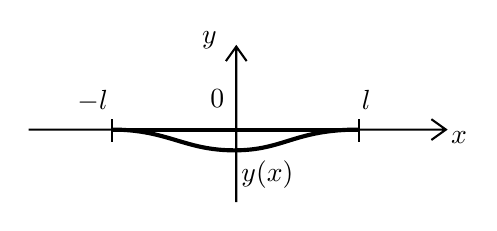
\begin{tikzpicture}[x=0.75pt,y=0.75pt,yscale=-1,xscale=1]
	%uncomment if require: \path (0,97); %set diagram left start at 0, and has height of 97
	
	%Shape: Axis 2D [id:dp059611853304774254] 
	\draw  (31,52) -- (232,52)(131,12) -- (131,87) (225,47) -- (232,52) -- (225,57) (126,19) -- (131,12) -- (136,19)  ;
	%Straight Lines [id:da1076030918406512] 
	\draw    (71,47) -- (71,58) ;
	%Straight Lines [id:da7590176182038997] 
	\draw    (190,47) -- (190,58) ;
	%Straight Lines [id:da7463067837936377] 
	\draw [line width=1.5]    (71,52) -- (190,52) ;
	%Curve Lines [id:da25330777154519524] 
	\draw [line width=1.5]    (71,52) .. controls (98,52) and (106,62) .. (130,62) .. controls (154,62) and (159,52) .. (190,52) ;
	
	% Text Node
	\draw (53,31.4) node [anchor=north west][inner sep=0.75pt]    {$-l$};
	% Text Node
	\draw (190,31.4) node [anchor=north west][inner sep=0.75pt]    {$l$};
	% Text Node
	\draw (117,31.4) node [anchor=north west][inner sep=0.75pt]    {$0$};
	% Text Node
	\draw (132,65.4) node [anchor=north west][inner sep=0.75pt]    {$y( x)$};
	% Text Node
	\draw (233,51.4) node [anchor=north west][inner sep=0.75pt]    {$x$};
	% Text Node
	\draw (113,3.4) node [anchor=north west][inner sep=0.75pt]    {$y$};
	
	
\end{tikzpicture} 

Балка жёстко закреплена на концах, поэтому кроме условия обычного закрепления $y(-l)=y(l)=0$ должно выполняться условие $y'(-l)=y'(l)=0$. В положении равновесия у балки будет минимальное значение потенциальной энергии. Когда происходит прогиб балки, то потенциальная энергия за счёт силы тяжести уменьшается, так как уменьшается ордината центра тяжести, и увеличивается за счёт появления изгибающего момента. Запишем полное выражение потенциальной энергии балки без вывода
\begin{equation}
	\label{l2:eq:19}
	\hfill E[y]=g\cdot\int\limits_{-l}^{+l}\rho\cdot\sqrt{1+y^{\prime2}}\cdot y\,dx+\frac12\cdot\int\limits_{-l}^{+l}\frac{\mu\cdot y''}{\left(1+y^{\prime2}\right)^{3/2}}\,dx.\hfill
\end{equation}
Здесь $g$ --- ускорение силы тяжести, $\rho$ --- плотность на единицу длины балки, $\mu$ --- коэффициент, описывающий упругие свойства балки. Так как её прогиб, очевидно, не большой, то $|y'|\ll1$. Поэтому в \eqref{l2:eq:19} можно пренебречь членом $y^{\prime2}$ и таким образом окончательно мы приходим к задаче:
\begin{multline*}
	\text{Найти }\min\limits_{y\in\K}\,E[y], \text{ где } E[y]=\int\limits_{-l}^{+l}\left(g\cdot\rho\cdot y+\frac{1}{2}\mu\cdot y^{\prime\prime}\right)\,dx,\\ \K=\left\{y(x)|y\in\Cfn[{[a,b]}]{2},\ y(l)=y'(l)=y(-l)=y'(-l)=0\right\}_{\displaystyle.}
\end{multline*} 
После построения общей теории мы вернёмся к этой задаче и решим её.  